\section{Studies with Experimental Data}

The neural network architecture tested on simulated data was used to train a neural network using real experimental data. As in our simulation studies, the pulses that are measured in one detector are very similar in width due to the same material with the same relaxation time and the same photo-multipliers with the same amplifiers. For our studies, we used pulse data from the Electromagnetic Calorimeter of CLAS12 detector, which makes up about $25\%$ of the data volume produced by CLAS12 data acquisition. 


\begin{figure}[h!]
\centering
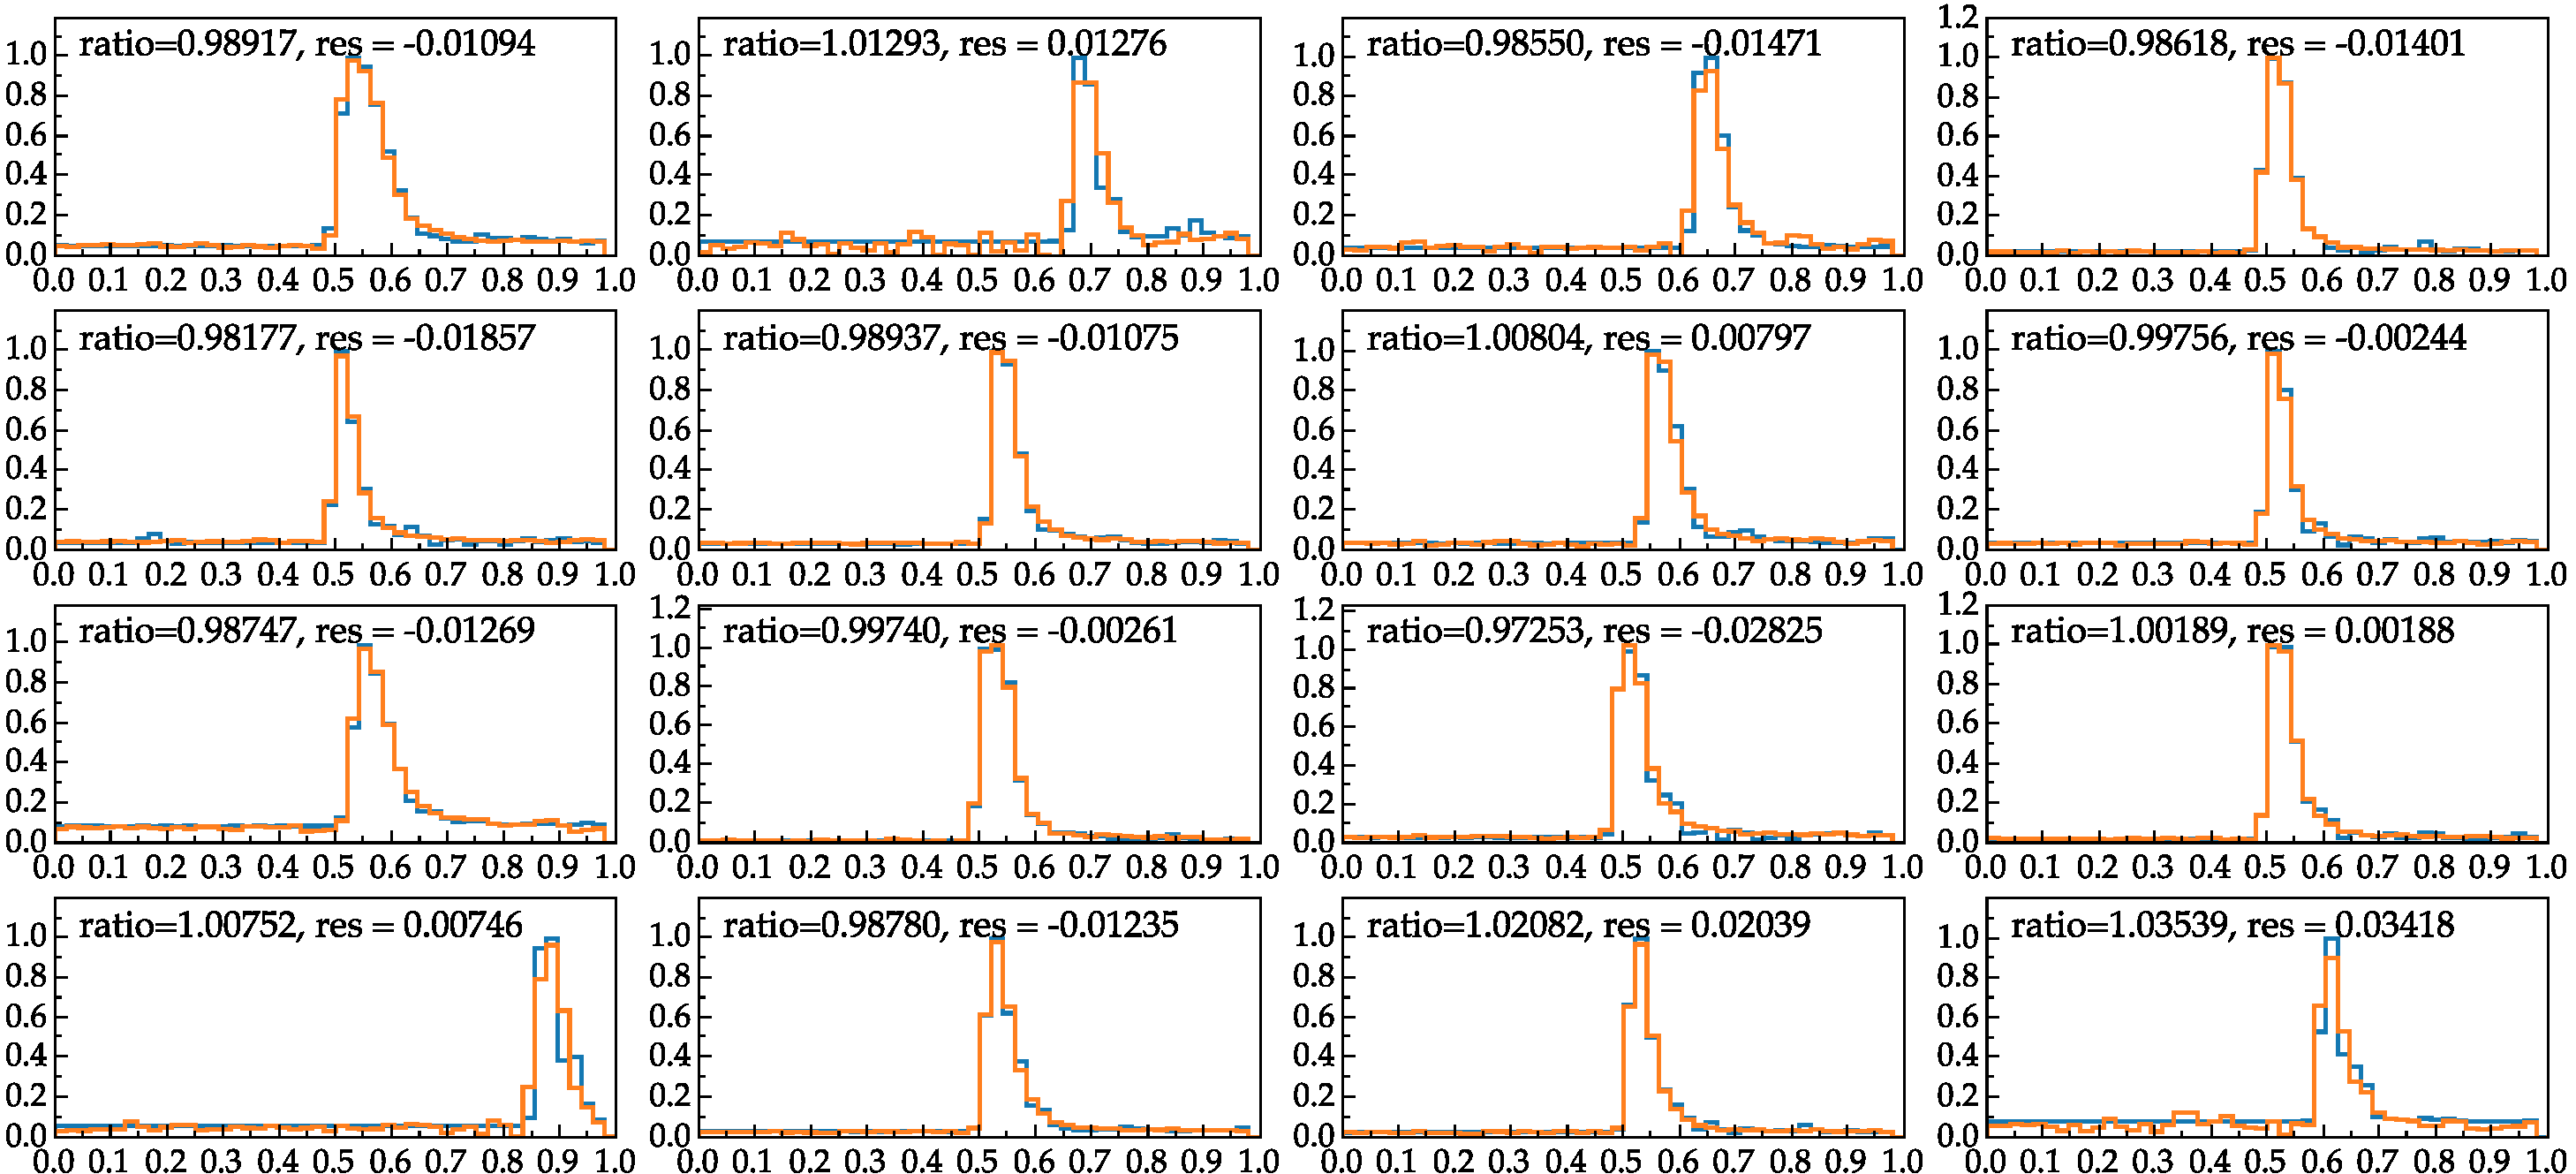
\includegraphics[width=0.95\columnwidth]{results_data_96.pdf}
\caption{Experimental data pulses plotted with the decompressed pulses overlayed. The compression is done with the improved auto-encoder [48,96,48,24,12,24,48.96,48] architecture. } 
\label{fig:results_data_96}
\end{figure}

\begin{figure}[h!]
\centering
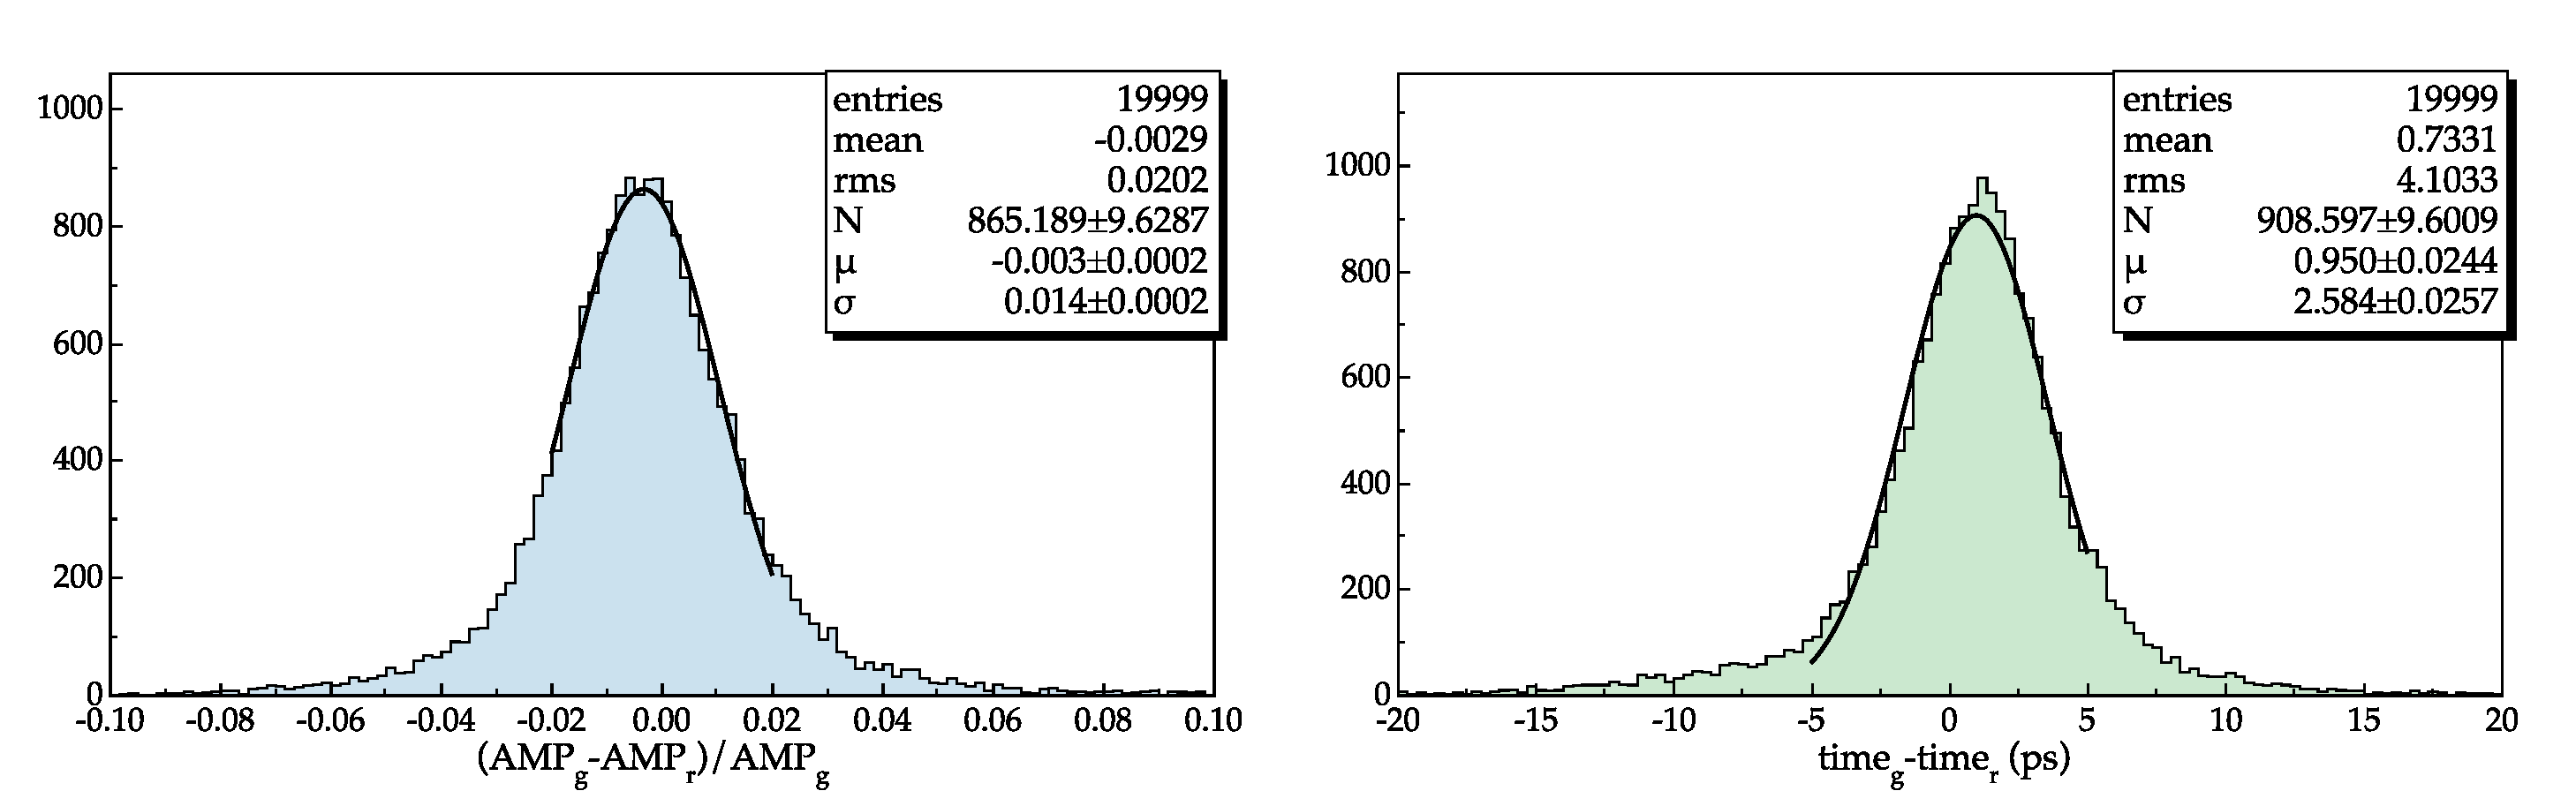
\includegraphics[width=0.9\columnwidth]{out_evaluate_csv_raw_96.pdf}
\caption{Resolution of the experimental pulses decompressed. Pulse amplitude resolution (on the left) and pulse timing resolution (on the right). } 
\label{fig:results_data_96_res}
\end{figure}

